\documentclass[12pt,spanish]{article}
\usepackage[spanish]{babel}
\usepackage{tikz}
\usepackage{graphicx}
\usetikzlibrary{matrix,backgrounds,babel}
\usepackage{texdraw}
\usepackage{subcaption}
\usepackage{multirow}
\usepackage[hidelinks]{hyperref}
\usepackage{caption}
\usepackage{multicol}
\usepackage[outputdir=build]{minted}
\usepackage[skins,minted,breakable]{tcolorbox}
\usepackage{float}
\usepackage{array}
\graphicspath{ {../img/} {../../LaTeX/img/} {/home/csp98/latex/img/}}
\selectlanguage{spanish}
\usepackage[utf8]{inputenc}
\usepackage{graphicx}
\usepackage[a4paper,left=2cm,right=2cm,top=2.5cm,bottom=2.5cm]{geometry}
\newtheorem{ppio}{Principio }

\newmintedfile[cppcode]{c++}{
linenos=true,
breaklines=true,
tabsize=2,
}

\newmintedfile[script]{bash}{
linenos=true,
breaklines=true,
tabsize=2,
}

\makeindex

\begin{document}
\begin{titlepage}

\newlength{\centeroffset}
\setlength{\centeroffset}{-0.5\oddsidemargin}
\addtolength{\centeroffset}{0.5\evensidemargin}
\thispagestyle{empty}

\noindent\hspace*{\centeroffset}
\begin{minipage}{\textwidth}

\centering
\includegraphics[width=0.9\textwidth]{logo_ugr.jpg}\\[1.4cm]

\textsc{ \Large Algorítmica\\[0.2cm]}
\textsc{GRADO EN INGENIERÍA INFORMÁTICA}\\[1cm]

{\Huge\bfseries Práctica 4\\}
\noindent\rule[-1ex]{\textwidth}{3pt}\\[3.5ex]
{\large\bfseries El viajante de comercio}
\end{minipage}

\vspace{1.5cm}
\noindent\hspace*{\centeroffset}
\begin{minipage}{\textwidth}
\centering

\textbf{Autores}\\ {María Jesús López Salmerón \\ Nazaret Román Guerrero \\ Laura Hernández Muñoz \\ José Baena Cobos  \\ Carlos Sánchez Páez}\\[2.5ex]
\includegraphics[width=0.3\textwidth]{etsiit_logo.png}\\[0.1cm]
\vspace{1.5cm}
\includegraphics[width=0.5\textwidth]{decsai.jpg}\\[0.1cm]
\vspace{1cm}
\textsc{Escuela Técnica Superior de Ingenierías Informática y de Telecomunicación}\\
\vspace{1cm}
\textsc{Curso 2017-2018}
\end{minipage}
\end{titlepage}
\tableofcontents
\thispagestyle{empty}
\listoffigures
\newpage
\setcounter{page}{1}
%%%%%%%%%%%%%%%%%%%%%%%%Comienzo del documento%%%%%%%%%%%%%%%%%%%%%%%%%%%%%%%
\section{Descripción de la práctica}

El objetivo de esta práctica es abarcar el problema del viajante de comercio (TSP, \textit{Travel Salesman Problem}) mediante estrategias voraces. En concreto, seguiremos la heurística de \textit{Branch and Bound}.\\

Tiene las siguientes características:
\begin{itemize}
	\item \textbf{Conjunto de candidatos}. Ciudades a visitar.
	\item \textbf{Conjunto de seleccionados}. Aquellas ciudades que vayamos incorporando al circuito.
	\item \textbf{Función solución}. Todas las ciudades han sido visitadas y hemos vuelto a la primera.
	\item \textbf{Función de factibilidad}. La ciudad no ha sido visitada aún.
	\item \textbf{Función selección}. De entre todos los candidatos, elegimos aquella ciudad que incrementa menos el coste del circuito que llevamos hasta el momento. 
\end{itemize}

\section{Descripción del algoritmo}

\subsection{Datos y estructuras utilizadas}

\begin{itemize}
	\item \textbf{Distancia}. Comienza inicializada a +$\infty$.
	\item \textbf{Cota inferior}. Utilizamos una cota inferior optimista que inicializamos mediante un algoritmo greedy, aproximado al algoritmo \textit{vecino más cercano}. La heurística que sigue el algoritmo es la siguiente:

\[
\centering \frac{1}{2} \sum_{i=0}^{n}coste_{entrada}(i)+coste_{salida}(i)
\]

En la sumatoria se acumulan progresivamente los costes de entrada y de salida de cada nodo que sean menores entre las aristas posibles de cada uno. Tras completar la sumatoria se divide a la mitad debido a que la salida de un nodo es la entrada del siguiente.
	\item \textbf{Solución parcial}. Es un vector que contiene la solución, pudiendo o no estar completa. En el caso de que esté completa pasa a ser la nueva cota.
	\item \textbf{Visitados}. Es un vector de booleanos que contiene \textit{true} si la ciudad ya ha sido visitada y \textit{false} en otro caso.

\end{itemize}

\subsection{Procedimiento}

El ajuste inicial que se lleva a cabo es el siguiente:

\begin{enumerate}
	\item Se calcula la cota inferior inicial mediante el algoritmo greedy anteoriormente explicado.
	\item Se toma la primera ciudad y se introduce en la solución parcial. La ciudad ya ha sido visitada, por tanto se pone a \textit{true} en el vector de visitados.
	\item Se llama entonces al método recursivo que lleva a cabo el algoritmo \textit{Branch and Bound} propiamente dicho.

\end{enumerate}

El seguimiento del algoritmo es el que sigue:

\begin{enumerate}
	\item En el caso base se comprueba si hemos llegado a un nodo hoja del árbol. Si efectivamente estamos en un nodo hoja, cerramos el circuito y comprobamos si la solución parcial actual es mejor que la global (la distancia es menor). En caso afirmativo, ésta se actualiza.
	\item Si no estamos en el caso base, se siguen los siguientes pasos
	\begin{enumerate}
		\item Recorremos todas las ciudades restantes.
		\item Comprobamos que no ha sido visitada y que no es la misma ciudad en la que estamos actualmente.
		\item Calculamos el coste que supone añadir la nueva ciudad al recorrido.
		\item Calculamos la cota de la rama actual. Se puede calcular de dos formas: si el nivel es el 1 la calculamos como la media entre el menor arco entrante de la última ciudad de la solución parcial y la nueva que queremos añadir. Si el nivel no es el 1, se calcula como la media entre el menor arco saliente de la última ciudad de la solución parcial y el menor arco entrante de la ciudad a añadir.
		\item Comprobamos si la suma entre la cota actual y el peso actual es menor que la distancia total, hemos encontrado una cota menor y por tanto exploramos los hijos mediante una llamada recursiva.
		\item Deshacemos los cambios que hemos realizado para que el siguiente hijo que evaluemos encuentre las variables en las mismas condiciones que el que se acaba de comprobar.
	\end{enumerate}
\end{enumerate}

\section{Resultados obtenidos}

\begin{figure}[H]
\centering
\begin{tabular}{|c|c|}
\hline
\textbf{Número de ciudades} & \textbf{Tiempo(s)}\\
\hline
6 & $3.3886 \cdot 10^{-5}$\\
\hline
7 & 0.000140369\\
\hline
8 & 0.000602488\\
\hline
9 & 0.00357393\\
\hline
10 & 0.0154363\\
\hline
11 & 0.128727\\
\hline
12 & 0.658938\\
\hline
13 & 4.02953\\
\hline
14 & 31.2847\\
\hline
15 & 245.842 (4 minutos y 5.842 segundos)\\
\hline
16 & 1541.08 (25 minutos y 41 segundos)\\
\hline
\end{tabular}
\caption{Tiempos obtenidos}
\end{figure}

\begin{figure}[H]
\centering
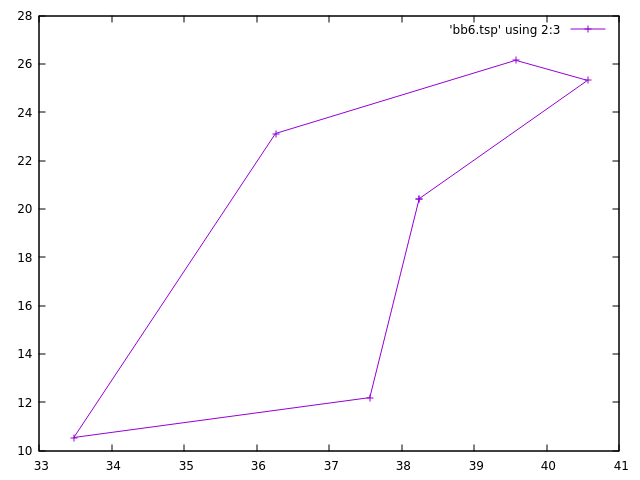
\includegraphics[scale=0.75]{bb6.png}
\caption{ulysses6.tsp}
\end{figure}

\begin{figure}[H]
\centering
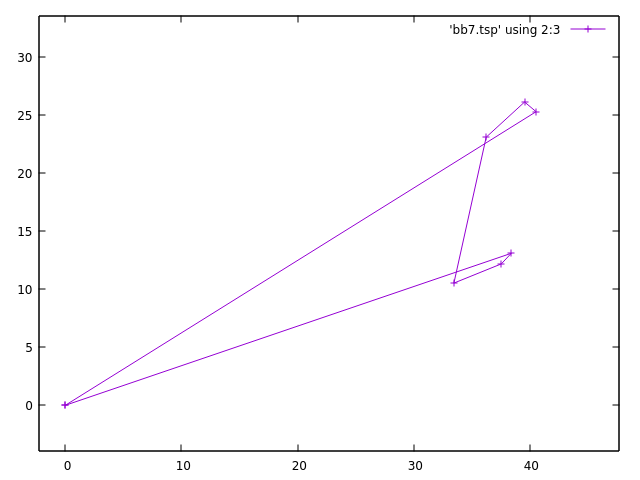
\includegraphics[scale=0.75]{bb7.png}
\caption{ulysses7.tsp}
\end{figure}

\begin{figure}[H]
\centering
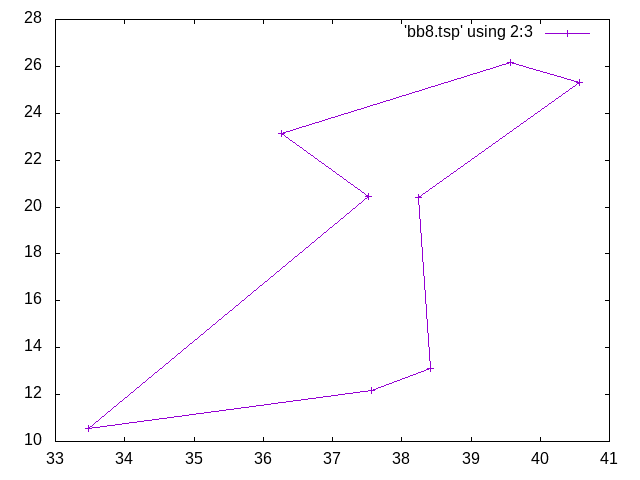
\includegraphics[scale=0.75]{bb8.png}
\caption{ulysses8.tsp}
\end{figure}

\begin{figure}[H]
\centering
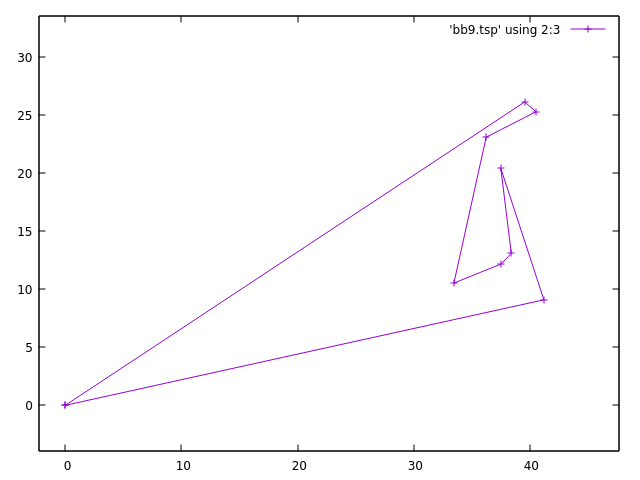
\includegraphics[scale=0.75]{bb9.png}
\caption{ulysses9.tsp}
\end{figure}

\begin{figure}[H]
\centering
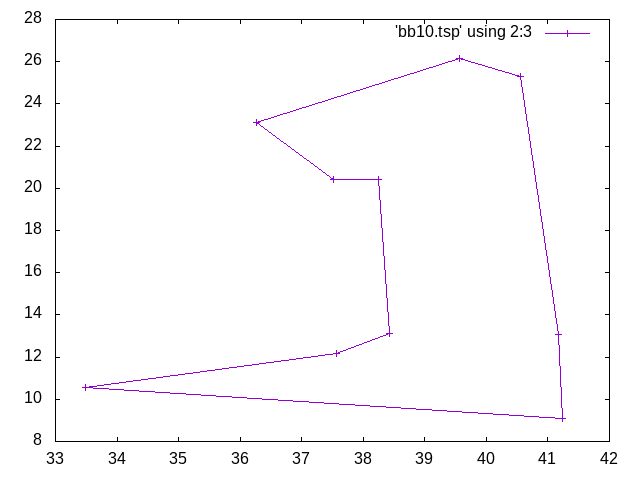
\includegraphics[scale=0.75]{bb10.png}
\caption{ulysses10.tsp}
\end{figure}

\begin{figure}[H]
\centering
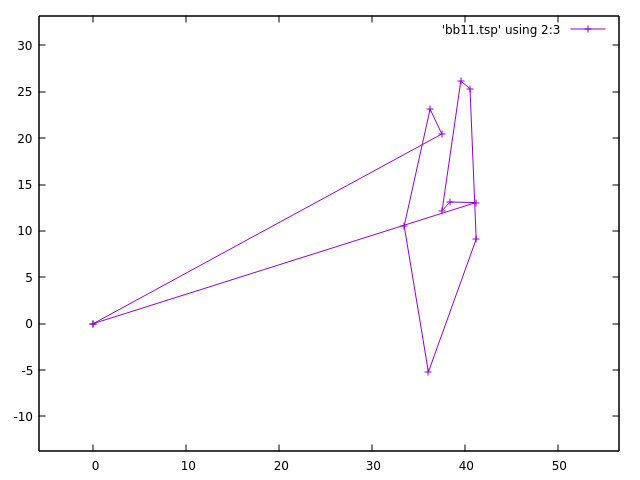
\includegraphics[scale=0.75]{bb11.png}
\caption{ulysses11.tsp}
\end{figure}

\begin{figure}[H]
\centering
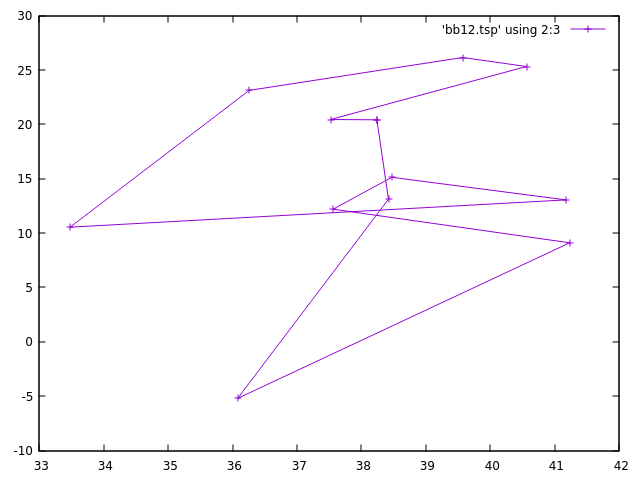
\includegraphics[scale=0.75]{bb12.png}
\caption{ulysses12.tsp}
\end{figure}

\begin{figure}[H]
\centering
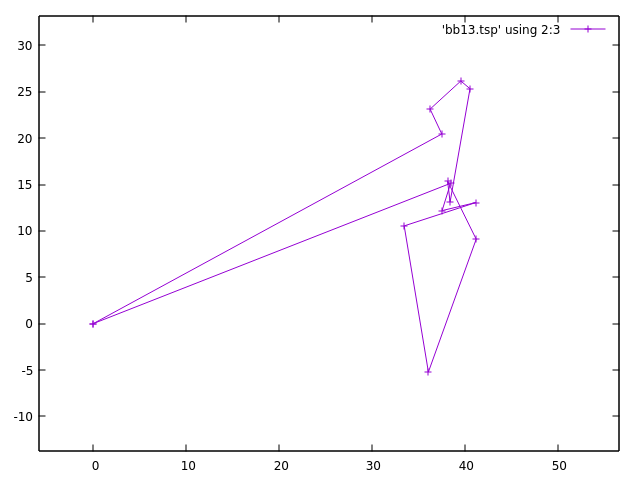
\includegraphics[scale=0.75]{bb13.png}
\caption{ulysses13.tsp}
\end{figure}

\begin{figure}[H]
\centering
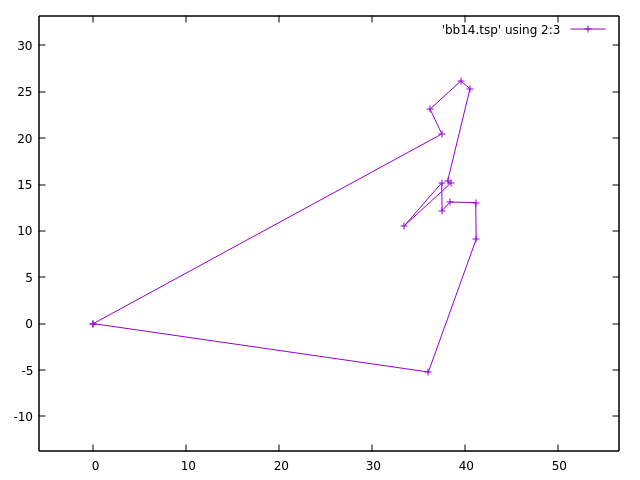
\includegraphics[scale=0.75]{bb14.png}
\caption{ulysses14.tsp}
\end{figure}

\begin{figure}[H]
\centering
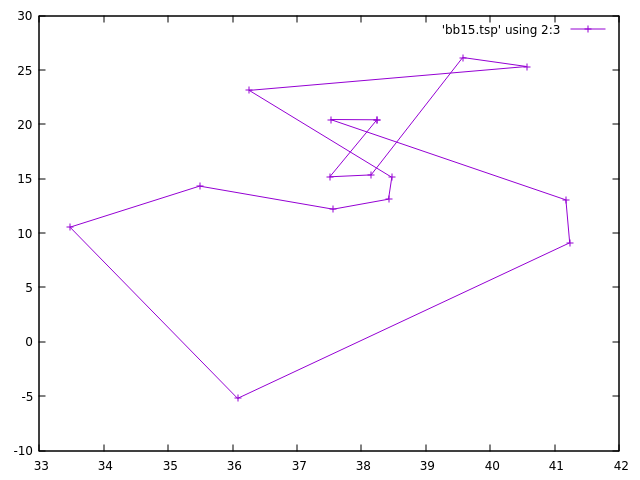
\includegraphics[scale=0.75]{bb15.png}
\caption{ulysses15.tsp}
\end{figure}

\begin{figure}[H]
\centering
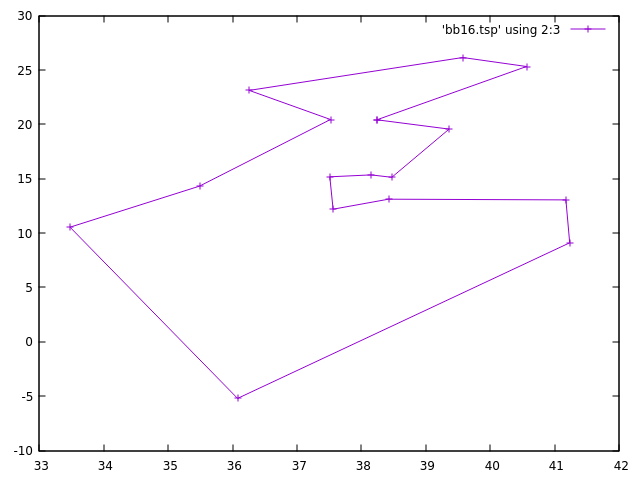
\includegraphics[scale=0.75]{bb16.png}
\caption{ulysses16.tsp}
\end{figure}

\begin{figure}[H]
\centering
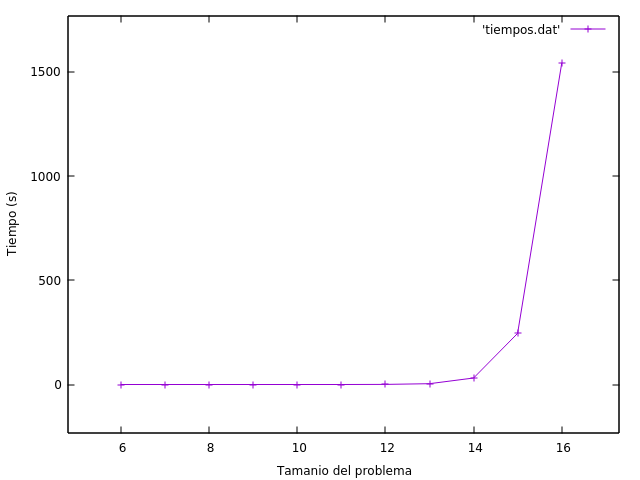
\includegraphics[scale=0.75]{tiempos.png}
\caption{Evolución del tiempo de ejecución}
\end{figure}


\section{Conclusiones}

Lo más destacable de este algoritmo es que en términos de orden de eficiencia es pésimo pero, sin embargo, proporciona una solución muy óptima.

\section{Anexo: código fuente}

\cppcode{tsp.cpp}
\captionof{figure}{TSP mediante Branch\&Bound}

\script{practica.sh}
\captionof{figure}{Ejecución de la práctica}

\script{gnuplot.sh}
\captionof{figure}{Generador de gráficas}

%%%%%%%%%%%%%%%%%%%%%%%%%%%%Fin del documento%%%%%%%%%%%%%%%%%%%%%%%%%%%%%%%%
\end{document}
